\chapterimage{prehiste.jpg} % Chapter heading image

\chapter{Preistoria}
\epigraph{Şi a fost seară şi a fost dimineaţă: ziua întâi.}{Genesis 1.5}
\section{Răsăritul omenirii. Un milion de ani pînă la era noastră}
Soarele african strălucea peste savana, peste marginea verde a junglei şi crestele de nisip al văii Oldoway. Aici colo se vedeau turme de antilope şi girafe. Masivi ca nişte munţi hoinăreau rinoceri gigantici, care nu se temeau nici de stăpânii savanei - machairodzi (tigrii cu dinţi ca sabia) şi leii cavernelor. Şi undeva aici, în junglele şi savanele din Africa de Est, locuite de strîmoşii oamenilor, maimute Australopithecus, care la fel de abil usrcau în copaci şi mergeau pe două picioare pe pamant. Nu prea înalţi, pîr îndesat, pielea inchisa la culoare şi fălci puternice. Ei aveau arme teribile pentru alte animale - măciuca, lovitura căreia era la fel de puternică ca lovitura labei de leu. Măciuca a fost prima invenţie a maimuţelor pe drumul lor spre dominaţia mondială. Apoi au urmat suliţa şi focul, ce lea dat stăpînire peste savană. Fluturînd suliţe şi torţe, vînătorii mînau turmele de antilope înebunite de groază către prăpastie - unde vânătorii cei mai experimentati omorau animale rănite. Apoi, se făcea un foc, unde erau prăjite de întregu animalele vînate. Rupeau cu mâinile carnea fierbinte... Sătui, urcau în peşterele şi aţipeau pînă a doua zi, pînă la vînătoarea următoare. 
\begin{wrapfigure}[10]{r}{0.3\linewidth} 
    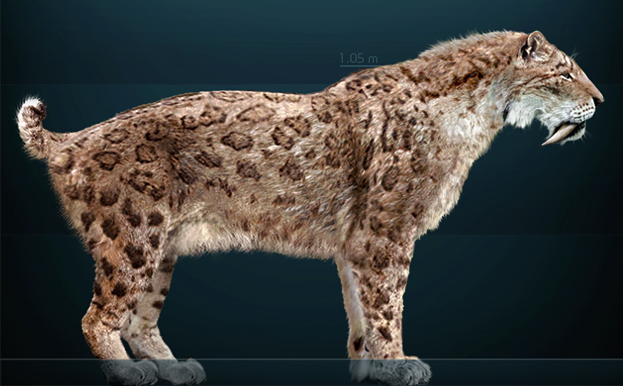
\includegraphics[width=0.4\textwidth]{mahaiord.jpg}
    \caption{Machairod (tigrul cu dinţi ca sabia) . Reconstrucţie grafică a Fatalis Smilodon bazat pe structurii osoase şi texte paleontologice.}
    \label{fig:pca}
\end{wrapfigure}

Nici rinocerii şi nici mamuţii uriaşi ce trăiau mai la nord nu puteu rezista turmele de maimuţe; cel mai temut duşman nu erau rinoceri sau leii, erau alte turme de maimuţe. În anii de foamete turmele vînau alte turme, toporele de piatră despicau craniile duşmanilor. Ca apoi câştigătorii, fluturând suliţe, ca de obicei, îi mînau pe cei învinşi în prăpastie. Ca întotdeauna, se făcea un foc şi se mînca prada, iar oasele învinşilor erau amesticate cu osele antilopelor vînate cîndva. 

Acest lucru a continuat din an în an, din secol în secol. Schimbarea climei, gheţarii care veneau de la nord, schimbarea întregii naturi au dus şi la schimbarea maimuţei; mîinile lor au devinit mai scurte, maxilarile mai mici şi capul a crescut în dimensiune. Australopithecus este substituit de Pithecanthropus,iar Pithecanthropus de Neanderthal, dar nu erau oamenii. Ele au rămas maimuţe - cu toate că s-au învăţat să se îmbrace în piei. Doar un miracol ar putea transforma o maimuţă într-un om. 
\subsubsection{Antropogeneza}
\epigraph{Triburile paleolitice au fost pline de tinereţe care nu se va mai întoarce, acea viaţă, energie şi putere pe care putem să ne o imaginăm cu greu.}{Joseph Henri Honoré Boex}

Preistoria constituie cea mai îndelungată perioadă din istoria umanităţii şi se înscrie, ca durată, de la primele manifestări ale prezenţei omului, atestate pe baza descoperirilor arheologice, până la descoperirea scrisului.

\begin{wrapfigure}[10]{l}{0.3\linewidth} 
    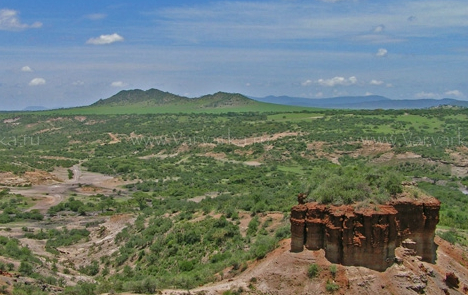
\includegraphics[width=0.3\textwidth]{oldoway.jpg}
    \caption{Valea Oldoway. Fotografie contemporană}
    \label{fig:pca}
\end{wrapfigure}
Istoria pune în prim plan geneza şi componenţa ei fundamentală, Omul. În timpul cuaternarului, în mai multe rânduri, s-au produs înaintări şi retrageri ale gheţarilor, corelate încă din 1874, de către J.Geikje, cu dezvoltarea culturilor paleolitice.

Antropogeneza studiază formarea şi dezvoltarea omului. Ea relevă trecerea omului din starea de animalitate în cea de umanitate, trecere condiţionată de trei coordonate esenţiale: starea bipedă, limbajul articulat şi gândirea. Locul şi data apariţiei omului pe Pământ este incertă.

Drumul spre sapientizare, respectiv către Homo Sapiens, a fost interpretat multă vreme din perspectiva evoluţionismului, evoluţia fiind considerată continuă şi ascendentă. Era contestată expresia biblică a genezei omului, într-o încercare de laicizare a gândirii, în două variante: fie omul se trage din maimuţă, fie sunt veri.

Descoperiri recente au pus în evidenţă şi alte posibilităţi de interpretare a genezei omului şi a raportului acestuia cu mediul geografic natural. Conform noii ipoteze, evoluţia este privită, în continuare în ascensiune, dar în spirală şi sinuoasă.

Dincolo de aceste ipoteze, un fapt este cert: omul a devenit o prezenţă activă într-un mediu  care, fără a-l favoriza în mod deosebit, nu i-a fost niciodată ostil.

Întemeiată pe studii etnografice asupra unor populaţii arhaice contemporane, ideea unei aşa-zise “vârste de aur” a umanităţii câştigă tot mai mulţi adepţi, lăsând în urmă, justificat în numeroase privinţe mitul omului neajutorat.

Pentru acest nivel de dezvoltare, persistenţa ideii de proprietate comună, absolută nu-şi mai are, nici ea, puncte de susţinere: delimitarea grupelor de vârstă, existenţa deosebirilor natural-biologice, statutul aparte, într-o comunitatea, al fiecărui membru al său, dezvăluie existenţa şi manifestarea simţului proprietăţii individuale.

În ceea ce priveşte începutul organizării sociale, trebuie regândită, din perspectivă, deosebirile dintre om şi lumea animală.

Direct sau indirect, mai mulţi factori au determinat fenomenul  răspândirii grupurilor umane pe Glob: schimbările geo-climatice, progresul tehnologic, capacitatea de adaptare a omului etc.

Dintr-o zonă restrânsă, între 1.800.000 - 900.000 este atestată o prezenţă generalizată a omului în întreaga Africă, Asia de sud, Europa de sud.

Aproximativ în acelaşi interval de timp (32.700 î.Hr.), grupe umane ating Australia.

America a fost şi ea populată prin strâmtoarea Behring, în timpul glaciaţiei Sartan (28.000-20.000 î.Hr.), în mai multe etape. Către neolitic sunt populate insulele Creta, Cipru şi Cicladele. Cu paleoliticul superior se constată un fenomen care îşi va pune amprenta asupra evoluţiei ulterioare a umanităţii: dezvoltarea mai accentuată a unor zone în raport cu altele care au evoluat tehnologic şi cultural mai puţin rapid.
\subsubsection{Dezvoltarea speciei umane}

\epigraph{Şi a zis Dumnezeu "Sa facem om după chipul şi dupa asemanarea noastră"}{Genesis 1.2}
Dezvoltarea omului din stamosii sai mai putin aratosi si inteligenti a avut loc in timpul ultimelor doua milioane de ani. Este probabil ca primul stadiu al acestei ramuri de evolutie organica, care a adus la ceea ce numim astazi Homo sapiens, sau omul care gandeste, sa fi inceput in Africa, in timpul pliocenului superior. In 1959, arheologul englez Louis Leakey a gasit in Africa de est resturile lui Zinjantropus, care se poate sa fi fost stra-stra-stra...bunicul nostru, al tuturor. Zinjantropus (numele inseamna omul est-african) a trait acum 1.750.000 ani si este cel mai vechi cioplitor de unelte de piatra pe care il cunoastem.

\begin{wrapfigure}[24]{r}{0.3\linewidth} 
    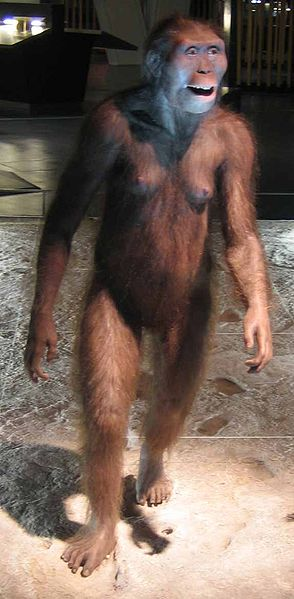
\includegraphics[width=0.3\textwidth]{austrolapitec.jpg}
    \caption{Reproduceri de Australopithecus afarensis în Cosmocaixa Barcelona.}
    \label{fig:pca}
\end{wrapfigure}
Fosilele lui australopitecus, omul-maimuta sud-african care a trait acum aproximativ 2.000.000 ani, au fost descoperite in 1920 de savantul englez Raymond Dart, impreuna cu arme de os si cu resturile animalelor ucise de el.

Din putinele urme de fosile descoperite reiese ca aceste fiinte cu aspect omenesc sau deplasat spre nord si spre est, raspandindu-se in toata Europa si Asia. In anul 500.000, pitecantropul traia pe insula Djawa si sinantropul in apropiere de actuala asezare a Peking-ului. Reprezentantii acestor doua genuri, care au disparut de mult, semanau foarte mult intre ei, ceea ce i-a facut pe antropologi sa-i includa intr-unul singur. Capacitatea lor craniana era de aproximativ 1000 centimetri cubi, in comparatie cu 1500 centimetri cubi, cat reprezinta cutia craniana a omului. Acesti indivizi, care erau destul de avansati pentru a-i putea considera stramosii nostri, aveau fruntea tesita si arcadele foarte pronuntate. Pitecantropul era familist, dar nu prea sociabil. El traia cu familia sa in padure si-si gasea adapost in pesteri. Se presupune ca se pricepea sa faca focul si sa-si construiasca obiecte simple si arme din lemn si piatra. Exista indicii ca acest tip de pre-om a trait si in Europa. Un maxilar gasit langa Heidelberg, in Germania se poate sa fi apartinut pitecantropului european.

Un stadiu mai avansat in evolutia omului il reprezinta omul de Neanderthal, ale carui ramasite se gasesc intr-un numar considerabil in Asia, Africa si Europa. Craniul sau era mai mare decat al pitecantropului, pe care il intreceau si ca indemanare. El era destul de scund si indesat, cu umerii incovoiati si genunchii usor indoiti, ca la maimutele de astazi. Fata sa era lata, fruntea joasa, cu arcadele proeminente; maxilarele semanau cu cele de animal, iar barbia era retrasa. Concurentul sau din alta ramura a rasei umane a fost omul de Cro-Magnon, numit astfel dupa pestera din apropierea micului sat Les Eyzies (sud-vestul Frantei), unde s-au gasit pentru prima oara resturile sale. Omul de Cro-Magnon era inalt brunet si chipes. Avea fruntea inalta, ceea ce dovedeste dezvoltarea partii frontale a creierului si barbia ascutita si proeminenta. Se pricepea foarte bine sa-si faca arme si sa vaneze, iar in timpul liber acoperea peretii cavernelor in care traia cu desene frumoase ale animalelor pe care le vana. Aceste desene pot rivaliza cu cele mai reusite picturi facute de oamenii moderni. E foarte probabil ca omul de Cro-Magnon stia sa vorbeasca si ca isi putea exprima emotiile si in muzica. Se prea poate sa fi existat o concurenta indarjita intre rasele Neanderthal si Cro-Magnon, cea din urma exterminand-o pe cea dintai. Astfel ajungem la omul de astazi. \footnote{O PLANETA NUMITA PAMANT, de George Gamow,Ed. Stiintifica, Buc. 1968, pag. 227 - 229} 

\subsection{Răsăritul omenirii. Patruzeci de mii de ani pînă la era noastră}
La fel strălucea peste savană soarele, la fel înverzeau copacii şi vîrfuri de munte străluceau la orizont.La fel se deplasau în lanţ pe câmpii vînătorii; dar în acest lanţ mergeau acum nu maimuţe dar oameni. Ei aveau aceleaşi topoare de piatră şi suliţe, dar nu arătau ca maimuţe. Ei erau înalţi, subţire şi vorbeau. Un miracol, unele mutaţie aleatoare au dus la faptul că a apărut primii oameni. 

Pentru un timp, oameni şi neanderthalienii trăiau unii lîngă alţii şi poate chiar se încălzeau la acelaş foc ca în peştera Tabun Cave din Palestina. Dar apoi sa întâmplat ceia ce trebuia să se întâmple: lipsa de alimente a generat între oameni şi neanderthalieni un război pe viaţă şi moarte. Gintele de oameni peste tot întâlneu neanderthalienii - stăpânii acestor locuri. Vînători mergînd în lanţ mînau neanderthalienii în prăpastie. Noile generaţii s-au mutat pese mişcau la sud, vest, est, avînd nevoie de noi terenuri. Ei urmăreau maimuţele izgoninindule în pădurii şi munţii. Peste zece mii de ani, cu neanderthalienii sa sfîrşit. Oameni au acaparat întreaga planeta. Doar unele popoare orientale, australieni şi ainu, au păstrat un mic amestec de sânge de Neanderthal - rezultatul amestecării învinşilor şi învingătorilor. 

A venit era de dominaţie a omului. Savanele, stepele şi tundra au fost împărţite între gintele de vânători. Deplasareaîndu-se mai departe spre nord, oamenii trecînd strâmtoarea încătuşată în geaţă au ajuns în America. Ei au populat un vast continent nou, pe care nu a călcat strămoşii lor- maimuţele. Chiar şi cei mai puternici nu au putut rezista noilor stăpîni ai lumii. Mamuţii uriaşi şi rinoceri au fost mînaţi în prăpastie la fel ca antilopele. Vînătorii dădeu foc la iarba şi soarteau la moarte tot ce era viu. Taberele lor au fost pline cu oasele de mii de bizoni şi cai. Mamuţii stângaci au fost sterşi de faţa pămîntului precum şi mastodonţi, cai americani şi zeci de alte specii. Oamenii ucideau animalele pentru a supravieţui. Ei deveneu mai mulţi la număr şi mai mult aveau nevoie de alimente. Ei populau pământul şi luau de la el tot ce puteau. Căutînd hrană - la fel ca şi strămoşii lor maimuţele - adunau plante comestibile. Apoi au învăţat cum să pescuiască, şi să se folosească de  năvod. Acum cincisprezece mii de ani, au inventat arcul ce a permis să vâneze păsări şi animale mici. Aceste descoperiri a fost o soluţie temporară, foamea se retrgea, ca apoi cînd populaţia crescu - se întorcea şi foametea. Anume ea impunea vînatul în lanţ a gintelor mai slabe. Arheologii astăzi găsesc în taberele vechi umane oase de mamuţi alături de oase de oameni. 

Omul era o parte a naturii - şi natura dicta legile ei crude.
\subsection{Omul şi natura}\index{Omul şi natura}
\epigraph{Populaţia este în mod inevitabil limitată de mijloacele de subzistenţă.}{Thomas Malthus}

Cu mult mai înainte decîtpînă cînd omul a devenit un stăpîn al planetei, leii dominau în savană. Leii, de asemenea, vânători  ca şi oamenii vînau în grup. După vânătoare împreună mâncau prada,  împreună aveau grijă de  puii şi trăiau într-o mare familie. Aveau teritoriul propriul şi luptau pentru el cu alte familii. Aceste lupte violente, mai devreme sau mai târziu sa încheiau cu moartea familiei.

Modul de viaţă a vînătorilor. Leoaica aduce în fiecare an mai mulţi puii care au nevoie de hrană; femeie dă viaţă copiilor care vor să mînînce. În ultimii ani, populaţia lumii a crescut cu doi la suta pe an, şi se poate presupune că numărul vînătorilor din acea perioadă creştea aproximativ la fel. În acest caz, ginta vînătorilor în jumătate de secol va creşte de 2,7 ori, iar pentru un secol - aproximativ de 7 ori. Vă puteţi imagina ce s-ar întîmpla în secolul următor? Peste două sute de ani numărul vînătorilor va creşte de 52 de ori, iar peste patru sute de anii - de 2700 de ori! Desigur, aceste nenumărate generaţii noi nu au suficientă mîncare şi un loc sub soare. Şi ei vor lupta pentru hrană - cu aceiaşi înverşunare ca şi leii.

Acestă forţă teribilă care îi mînă pe oamenii pe câmpul de luptă se numeşte \textbf{PRESIUNE DEMOGRAFICĂ}. Mai simplu, presiunea demografică - este foamea, adică mărimea învers proporţionară a consumului de alimente pe cap de locuitor. De exemplu, în Europa consumul de alimente este de două ori mai mare ca în India - aceasta înseamnă că presiunea demografică în India este de două ori mai mare, ceea ce înseamnă că India este în pericol constant de foamete şi războaie interne.

Imaginaţi-vă un teritoriu care aparţine unei ginţi de vînştori: păşiuni cu turme de animele ce pasc,pădurii pline de ciuperici şi rădăcini comestibile, un rîu bogat în peşte. Tot acest teritoriu, cu resursele sale alimentare - aceasta este  \textbf{NIŞA ECOLOGICĂ} a gintei. În cazul în care ginta creşte, ea preseză pereţii aceastei nişe, încercînd să o lărgească. Nişa ecologică poate fi extinsă prin unele invenţii, ca exemplu un harpon pentru un pescuit mai efecient  - invenţie care lărgeşte nişa ecologică, denumite \textbf{DESCOPERIRI FUNDAMENTALE}. Arcul, săgeţi otravite şi  nimimicirea gintei vecine, acapărarea pămînturilor lor  -  de asemenea este extinderea nişei ecologice. Măciuca, focul, suliţa, toporul de piatră, arcul - toate acestea au fost descoperiri fundamentale care au permis maimuţelor şi oamenilor să extindă nişa lor ecologică. Efectuarea acestor descoperiri, omul, în acelaşi timp, se schimba şi el. Oobiceiurile şi comportamentul  se complică spre deosebire de cele  moştenite. Uneori aceste modificări pot fi atît de mari încît putem vorbi despre naşterea unei noi \textbf{SPECII UMANE}. De multe ori acestă nouă specie se dovedeşte a fi ostilă altor oameni. Creînd noi arme şi mînate de foame, ea a început un război împotriva lor pentru spaţiu de viaţă. Pe de altă parte, presînd pereţii nişei ecologice, ei la rândul său, a simţeu presiunea de răspuns - foamete, boli,  atacurile altor ginţ. Puterea totală a acestei presiunii poate fi măsurată prin pierderile aduse - rata mortalităţii a populaţiei adulte. Populaţia demografică se măsoară ca suma coeficientulul consumului de alimente cu coeficientul de decese din cauza foamei. Presiunea lumei inconjurătoare totdeuna avea chipul morţii. Pentru a se opune acestui etern pericol  a fost necesar să se unească într-o singură gintă sau trib. 

\textbf{ERA NECESAR DE A TRĂI ÎMPREUNĂ}

\section{Ginta}\index{Ginta}
\epigraph{Adunaţi-vă împreună!

Împreună înţelegiţi-vă!

Să fie un singur gînd, 

O inima singură să aveţi!}{Rigveda}

Ce înseamnă a trai împreuna? Aceasta înseamnă să mergem împreună  umăr la umăr în lupta sau la vinatoare. Acesta înseamnă la un foc de tabara să mininci cu totiu carne fierbinte şi în caz de necesitate, fără ezitare să dai partea ta prietenului sau fratelui dace ei au nevoie. 
\begin{quote}
"Eskimosi - a scris un celebru explorator polar Rasmussen - traesc într-un comunism este atât de pronunţat că nu există cote speciale de vânătoare. Toate mesele sunt comune cînd este ucis orice animal ...." 
\end{quote}


Comunismul. Egalitate. Fraternitate. Sunt tradiţii vânătorilor  din toate timpurile. Vînătorul nu putea trăi singur: sursă de alimentare în epoca piatrii a fost o vânătoare colectivă. Singuraticul era  condamnat la moarte. Luptînd pentru viaţă, oamenii se uneau - astfel încât fiecare simţea lîngă braţul său braţul prietenului apropiat sau braţul fratelui.

Ginta - aşa se numeşte marele întreg, care a apărut în urma uniunii corpurilor şi sufletelor. Toate bărbaţii gintei erau consideraţi fraţii şi fraternitatea nu depindea de circumstanţele de naştere. Bărbaţii-fraţi erau de nedespărţit, ei vînau împreună, mîncau împreună şi  dormeau împreună. Unitate lor ajungea la abnegare: fraţii sciţi jurau că, dacă este necesar, să moară unul pentru altul. "Şi noi într-adevăr aşa şi procedăm, - spunea scitul Toksaris, eroul unui scriitor antic. - Din momentul în care ne-am crestat degetele, şi picurăm sânge într-o cupă mai apoi cufundînd fîrful săbilor noastre, gustînd acest sînge şi nimic nu ne mai poate despărţi ".

Unitatea nu lasă loc pentru egoism şi răutate. Integritate, onestitate, deschidere au fost calităţile esenţiale ale vînătorului. "Dumnezeu a creat aceste persoane simple, fără nici un vicii şi şiretlic" - scria episcopu lspaniol  Las Casas despre indienii americani. Viclenia şi înşelăciunea năşteau neîncredere şi discordie, precum şi cele mai mici controverse în faţa pericolelor inconjurătoare  puteau duce la peire.

Oameni di Epoca de Piatră nu ştiau ce e  bogăţie şi putere. Membrii ginţiit erau  egali între ei şi împreună hotărau problemele comune. Căpetenile alese nu  aveau posibilităţi de a se exprima, pentru că nu a exista nici cearturi sau neînţelegeri, nu erau  cei pe care ar fi trebui să-i judece şi să-i pedepsească. Sancţiunea ce mai severă era  luarea în rîs publică a vinovatului - şi care era destul pentru ca el să-şi corecteze comportamentul sau să moară de ruşine. Ruşinea, teama de a fi ridicolizat  public, ambiţie - acestea sunt calitatile care ne-au lăsat moştenire  oamenii din epoca de piatră. Ambiţia la acel moment înlocuia bogăţia şi oamenii au fost dispuşi să îşi asume riscuri, pentru a primi de la rude cuvinte de laudă.

Unititatea era  mai presus de toate, nimic nu putea dezbina bărbaţii gintei: nici cearturi, nici partea din trifeele vînătoreşti, nici rivalitate din cauza femeilor. Căsătoria a existat formal: fiecare bărbat trebuia să-şi aducă în gintă  femeie care era soţia lui - prima lui soţie. Dar, aşa cum se obişnuieşlte printre australienii, fiecare bărbat avea, de asemenea, a doua a treia a patra soţie, - soţiile fraţilor. Aleuţi numesc soţia fratelui "Ayaganov" ("Soţia mea") sau "ayagatanah" ("Locţiitoarea soţiei"). Barbatii schimbau soţiile şi copiii lor  cu alţi bărbaţi - aproape jumătate din copiii eschimoşilor care trăiesc în Repulse Bay, cresc nu în familiile în care s-au născut. Prieteni, "tovarăşi de cîntec," chiar au formal soţii comune. Chiar şi acum, în multe ţări din Asia nu au uitat încă vechi obiceiul de a oferii oasepetelui soţia.

Permanentul schimb de femei, copii, alimente era completat cu schimbul de cadouri -  puţinul pe care îl aveau vînători în proprietate personală: cuţite de piatră, bumeranguri, centuri din păr uman. Ginta era unită, şi toate bunurile erau comune, lucru care se evidenţia în timpul sărbătorilor legate de naştere. Mese comune, rugăciunea către un strămoş comun, dansuri extatice şi dragostea dezordonată simboliza unitatea familiei. Ginta a fost întruchiparea unităţii şi numai unitate ar putea salva poporul în ceasul  grelelor încercări la vînat sau luptă.

\subsection{Viaţa gintei}\index{Viaţa gintei}
\epigraph{Uniţi de turme comune,

Uniţi de gînduri comune

Luptau împreună!}{Rigveda}

Barbaţii erau stăpînii acestei vieţi deoarece ei hrăţeau ginta - de la succesul lor la vînătoare depindea viaţa fiecăruia. Femeile rareori  participau la marele vînători, principalele ocupaţii fiind culesul şi hrănirea a copiilor. Bărbaţii piereau la vînătoare şi în războaie - deci femeile trebuiau să dea naştere la mai mulţi copii. Femeile  prolifice avea cel mai mare respect din partea bărbaţilori. Copiii erau mulţi, dar nu toţi erau crescuţi.  Numărul membrilor gintei era limitat de mărimea şi potenţialul teritoriului pe care-l populau. Copiii erau supuşi unei selecţii naturale şi artificiale. Cu cîţi mai mulţi copii s-au născut, cu atît mai rezistenţi şi puternic erau cei care  supravieţuiau până la maturitate.

Selectarea începea de la naştere: indienii scăldau copiii noi-născuţi în timpul iernii în apă rece. Uneori, în primele zile ei nu erau hrăniţi şi îmbrăcaţi. Selectarea se sfîrşea cu o iniţiere. Australieni explica aceste ritualuri  crude prin dorinţa de a reduce numărul populaţiei. Selecţia fetelor era  mai puţin strictă: fetele erau menite pentru schimb şi în cele din urmă părăseau părinţii. Deaorece se năşteau cu mult mai mult decît era necesară pentru schimb de, majoritatea fetelor nou-nascuti erau ucise. Fete ce se îmbolnăveau aleuţi le ucideau pînă la vîrsta de şase ani.

\subsection{Înaceputul Matriarhatului}\index{Înaceputul Matriarhatului}
\epigraph{Uniţi de turme comune,

Uniţi de gînduri comune

Luptau împreună!}{Rigveda}

Văduvele şi femeile în vîrstă erau înreţinute de gintă, care respecta experienţa lor de viaţă.Barbatii, de obicei, nu ajungeau la bătrîneţe, asa că deţinătorii de tradiţii şi secrete mistice, vrăjitorii  au fost de multe ori femeile. Bătrînele  puteau să dea un sfat bun, vindeca boli, dar şi putea să pună vraji, doar de a avea un fir de păr sau o unghie a victimei. Aceasta vrajă  de obicei, îl nimicea pe om, de îndată ce a aflat despre asta.

Vrăjitoarele puteau să "adulmece criminalul", să afle voinţa strămoşilor, se transformau în corb şi alungau păsările - spiritele rele. Dar ritualuri de vânătoare erau înfăptuite de obicei de samanii bărbaţi. Ei desenau conturul de animale şi cîntînd vrăji, le-a străpungeu cu suliţe. Uneori, vînători îmbrăcaţi în piei de animale, organizau cpectacole destul de sofisticate. Pe pereţii peşterilor pictau cai şi bizoni străpunşi de suliţe. Aceste desene formează un tablou întreg, cum ar fi celebra galerie din peşteră Montespan. \begin{wrapfigure}[24]{l}{0.3\linewidth} 
    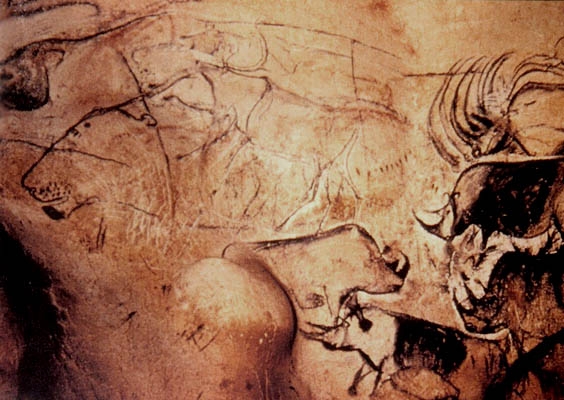
\includegraphics[width=0.3\textwidth]{montespan.jpg}
    \caption{Leii şi rinoceri din peştera Montespan. Fotografie de situl \url{https://github.com/LaurethTeX/Clustering} }
    \label{fig:pca}
\end{wrapfigure}